\subsection{The \texttt{LNSR:} module}

The {\tt LNSR:} module performs a single iteration of the line search algorithm, used as inner iteration of steepest descent,
conjugate gradient or quasi-Newton optimization techniques.\cite{recipie} The Armijo line search algorithm is used.\cite{armijo}
The {\tt LNSR:} module is generally used inside an inner loop, as depicted in Fig~\ref{fig:fig_lnsr}.

\vskip 0.2cm

\begin{figure}[h!]
\begin{center}
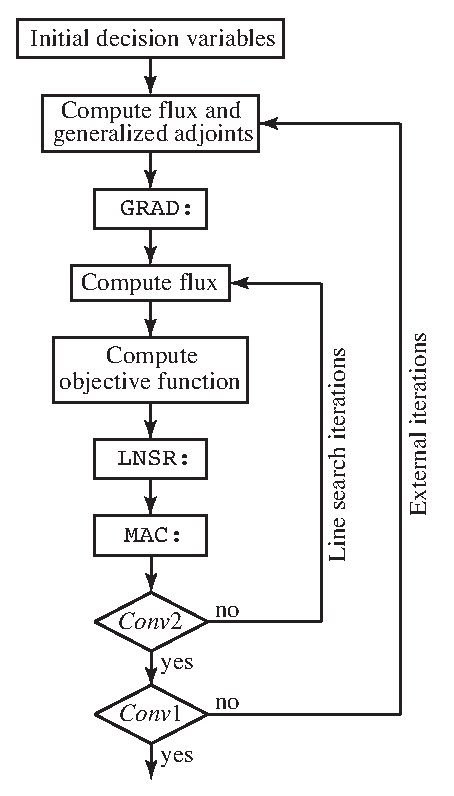
\includegraphics[scale=0.85]{Figures/lnsr.eps} 
\caption{Line search iterations.}\label{fig:fig_lnsr}
\end{center}
\end{figure}

The calling specifications are:

\begin{DataStructure}{Structure \moc{LNSR:}}
\dusa{OPTIM} \moc{:=} \moc{LNSR:} \dusa{OPTIM} \moc{::} \dstr{lnsr\_data}
\end{DataStructure}

\noindent where

\begin{ListeDeDescription}{mmmmmmmm}

\item[\dusa{OPTIM}] \texttt{character*12} name of the \dds{optimize} object ({\tt L\_OPTIMIZE} signature) containing the
optimization informations. Object \dusa{OPTIM} must appear on both LHS and RHS to be able to update the previous values.

\item[\dstr{lnsr\_data}] structure containing the data to the module \texttt{LNSR:} (see Sect.~\ref{sect:lnsr_data}).

\end{ListeDeDescription}
\vskip 0.2cm
\goodbreak

\subsubsection{Data input for module \texttt{LNSR:}}\label{sect:lnsr_data}

\begin{DataStructure}{Structure \moc{lnsr\_data}}
$[$ \moc{EDIT} \dusa{iprint} $]$ \\
$[~\{$ \moc{MAXIMIZE} $|$ \moc{MINIMIZE} $\}~]$ \\
$[$ \moc{OUT-STEP-LIM} \dusa{sr} $]$ \\
$[$ \moc{OUT-STEP-EPS} \dusa{$\epsilon_{ext}$} $]~[$ \moc{INN-STEP-EPS} \dusa{$\epsilon_{inn}$} $]$ \\
\moc{OUT-ITER-MAX} \dusa{maxE} \\
$[$ \moc{OUT-RESTART} \dusa{nstart} $]$ \\
$[~\{$ \moc{SD} $|$ \moc{CG} $|$ \moc{BFGS} $|$ \moc{LBFGS} $[$ \moc{hist\_nr} $]~|$ \moc{NEWT} $\}~]$ \\
$[$ \moc{INN-CONV-TST} {\tt >>} \dusa{$l_{convI}$} {\tt <<}  \moc{OUT-CONV-TST} {\tt >>} \dusa{$l_{convE}$} {\tt <<} $]$ \\
;
\end{DataStructure}

\noindent where
\begin{ListeDeDescription}{mmmmmmmm}

\item[\moc{EDIT}] keyword used to set \dusa{iprint}.

\item[\dusa{iprint}] index used to control the printing in module.

\item[\moc{MAXIMIZE}] keyword used to specify that the optimization problem will be a maximization.

\item[\moc{MINIMIZE}] keyword used to specify that the optimization problem will be a minimization (default).

\item[\moc{OUT-STEP-LIM}] keyword used to set or reset the maximum stepsize for the line search (default value is \dusa{sr} $=1.0$
or the value recovered from \dusa{OPTIM}).

\item[\dusa{sr}] initial radius of the stepsize (real or double precision).

\item[\moc{OUT-STEP-EPS}] keyword used to set the tolerance of outer iteration convergence inside module {\tt LNSR:} (default value
is $1.0 \times 10^{-4}$).

\item[\dusa{$\epsilon_{ext}$}] tolerance value (real or double precision).

\item[\moc{INN-STEP-EPS}] keyword used to set the tolerance used for the line search algorithm (default value
is $1.0 \times 10^{-4}$).

\item[\dusa{$\epsilon_{inn}$}] tolerance value (real or double precision).

\item[\moc{OUT-ITER-MAX}] keyword used to set the maximum number of external iterations.

\item[\dusa{maxE}] maximum number of external iterations.

\item[\moc{OUT-RESTART}] keyword used to set the external iteration restart cycle. A new recursion cycle
is restarted from the conjugate gradient method. By default, no restart is performed.

\item[\dusa{nstart}] number of iterations in one external iteration restart cycle.

\item[\moc{SD}] steepest descent method (default option).

\item[\moc{CG}] conjugate gradient method.

\item[\moc{BFGS}] Broyden-Fletcher-Goldfarb-Shanno method.\cite{recipie}

\item[\moc{LBFGS}] Memory limited Broyden-Fletcher-Goldfarb-Shanno method.\cite{nocedal}

\item[\dusa{hist\_nr}] number of corrections used in the memory limited Broyden-Fletcher-Goldfarb-Shanno method (default value
is 10).

\item[\moc{NEWT}] Newton method for unconstrained optimization.\cite{sph1981}

\item[\moc{INN-CONV-TST}] keyword used to determine if the line search convergence has been reached.

\item[\dusa{$l_{convI}$}] $=1$ means that line search convergence has been reached; $=0$ otherwise.

\item[\moc{OUT-CONV-TST}] keyword used to determine if the external convergence has been reached.

\item[\dusa{$l_{convI}$}] $=1$ means that external convergence has been reached; $=0$ otherwise.

\end{ListeDeDescription}
\clearpage
